\documentclass{article}

\usepackage{lmodern}
\usepackage[T1]{fontenc}
\usepackage[spanish,activeacute]{babel}
\usepackage{mathtools}
\usepackage{graphicx}


\title{TEMA 1 DESARROLLO DE SOFTWARE}
\author{Antonio Muñoz Cubero}
\date{1 de Ocutbre de 2020} 


\begin{document}
\maketitle
\pagenumbering{gobble}


Resumen del Tema 1 (Desarrollo de Software) para la asignatura Entornos de Desarrollo en el 
I.E.S Francisco de los Rios para el Grado Superior de Desarrollo de Aplicaciones Multiplataforma
\\
\\
\\
\\
\\
\\
\\
\\
\\
\\
\\
\\
\\
\\
\\
\\
\\
\\
\\
\\
\\
\\
\\
\\
\\
\\
\\

\includegraphics[width=1\linewidth]{cabecera_50_aniversario.png}
\newpage
\pagenumbering{roman}

\section{Introducción}
\subsection{¿Qué es un Software?}

Conocemos como \textbf{\textit{Sofware}} al soporte lógico de un sistema infomático, que comprende el cunjunto de los
componentes lógicos necesarios que hacen posible la realización de tareas específicas, en contraposición
los componentes físicos que son nombrados \textit{"Hardware"}.\\

La interación entre el \textbf{\textit{Sofware}} y el \textit{Hardware} hace operativo a un ordenador o cualquier otro 
dispositivo, es decir, el \textbf{\textit{Sofware}} envía instrucciones que el \textit{Hardware} ejecuta, haciendo posible 
el correcto funcionamiento de la máquina utilizada.\\

El \textbf{\textit{Sofware}}, en su mayoria, está escrito en lenguajes de programación de alto nivel, ya que son más fáciles
y eficientes para que los programadores los usen, ya que son los más cercanos al lenguaje natural respecto al lenguaje máquina.
Los lenguajes de alto nivel se traducen a lenguaje máquina para que esta la interprete y realice las acciones descritas en el código
\textbf{\textit{Sofware}} de alto nivel, usando bien un compilador o un interprete (algunos lenguajes necesitan de un híbrido de ambos).

\section{Ciclo de vida Sofware}
Un proceso de software es el conjunto de actividades necesarias para transformar los requisitos de un usuario en un sistema software. 
Cuando implica la construcción de un producto, se suele llamar ciclo de vida e incluye el periodo de tiempo comprendido desde la definición 
de los requisitos hasta el fin de su uso. El ciclo de vida presenta unos procesos primarios, como se reflejan en la siguiente imagen.
\\

\begin{figure}[b]
   
    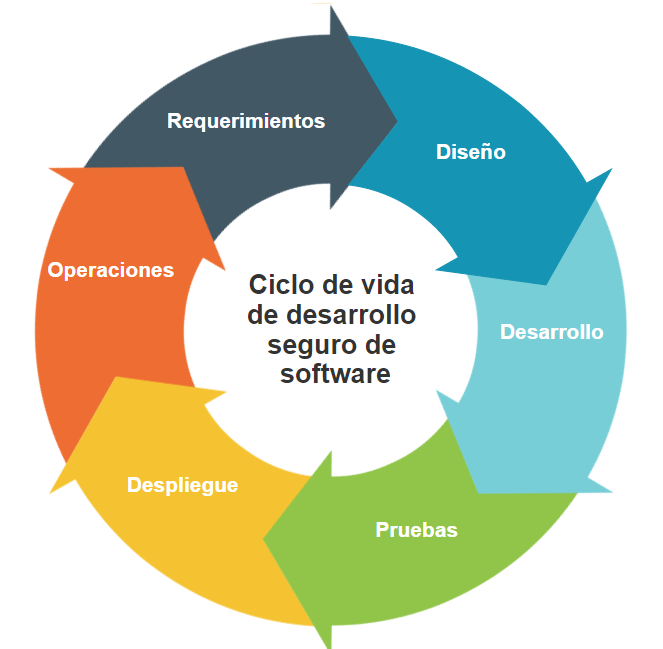
\includegraphics[scale=0.22]{Software-Development-Life-Cycle.png}
    \centering
    
\end{figure}

\newpage
\section{Fases del Desarrollo Sofwaer}
La aplicación de procesos, tanto en el desarrollo como en el posterior mantenimiento y operación del software siguen unos “patrones fijos” 
que configuran el esquema de mapa de situación, relación y continuidad entre los diferentes procesos, actividades y tareas. La etapa de 
desarrollo da paso al ciclo de vida del sistema y en las diferentes etapas del ciclo de vida pueden intervenir modificadores.


\end{document}



